\documentclass{article}
\usepackage{tikz}
\begin{document}
The original map look as following, violet squares are the location where a
secret door might be found.

\begin{center}
  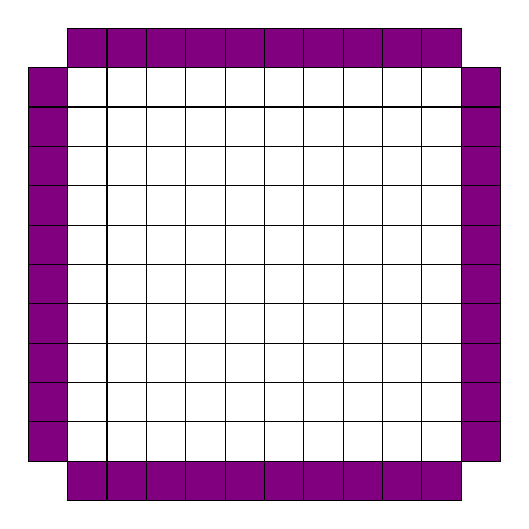
\begin{tikzpicture}[scale=.5]
    % Drawing Walls part
    \foreach \x in {1,...,10}{
      \draw [fill=violet] (\x,  0) rectangle (\x + 1,  1);
      \draw [fill=violet] (\x, 11) rectangle (\x + 1, 12);
    }
    \foreach \y in {1,...,10}{
      \draw [fill=violet] ( 0, \y) rectangle ( 1, \y + 1);
      \draw [fill=violet] (11, \y) rectangle (12, \y + 1);
    }
    % Drawing internal grid
    \foreach \x in {1,...,10}{
      \foreach \y in {1,...,10}{
        \draw (\x,\y) rectangle (\x + 1,\y + 1);
      }
    }
  \end{tikzpicture}
\end{center}

It is possible to fix some squares where research would be performed, trying to
use the lowest number of squares and avoiding two possible research on the
same square \footnote{This notion is close to the notion of domination set in
graph theory}. We can then obtain following result, with the filled orange squares
being the squares where research would be performed. And the empty orange squares
being the range of research.

\begin{center}
  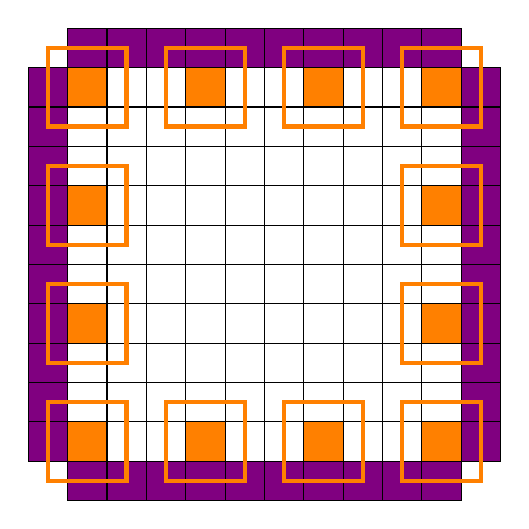
\begin{tikzpicture}[scale=.5]
    % Drawing Walls part
    \foreach \x in {1,...,10}{
      \draw [fill=violet] (\x,  0) rectangle (\x + 1,  1);
      \draw [fill=violet] (\x, 11) rectangle (\x + 1, 12);
    }
    \foreach \y in {1,...,10}{
      \draw [fill=violet] ( 0, \y) rectangle ( 1, \y + 1);
      \draw [fill=violet] (11, \y) rectangle (12, \y + 1);
    }
    % Drawing internal grid
    \foreach \x in {1,...,10}{
      \foreach \y in {1,...,10}{
        \draw (\x,\y) rectangle (\x + 1,\y + 1);
      }
    }
    % Coloring squares and ranges of research
    \foreach \x in {1,4,7,10}{
      \draw [fill=orange] (\x,  1) rectangle (\x + 1,  2);
      \draw [fill=orange] (\x, 10) rectangle (\x + 1, 11);
      \draw [ultra thick, orange] (\x - 0.5, 0.5) rectangle (\x + 1.5,  2.5);
      \draw [ultra thick, orange] (\x - 0.5, 9.5) rectangle (\x + 1.5, 11.5);
    }
    \foreach \y in {1,4,7,10}{
      \draw [fill=orange] ( 1, \y) rectangle ( 2, \y + 1);
      \draw [fill=orange] (10, \y) rectangle (11, \y + 1);
      \draw [ultra thick, orange] (0.5, \y - 0.5) rectangle ( 2.5, \y + 1.5);
      \draw [ultra thick, orange] (9.5, \y - 0.5) rectangle (11.5, \y + 1.5);
    }
  \end{tikzpicture}
\end{center}

Obviously, it's impossible to cover each square with a potential secret door
with less squares, because all the corners are used and there isn't any square
being ``covered'' by two different squares. If we ignore the cost of moves,
considering only the cost of research, the best policy seems to be always
looking first in the corners and after in the other spots, if all have the same
number of research at starts. But it's not obvious that the chance of finding a
secret door in a corner with $n+1$ researches is always lower than the chance
of finding a secret door in a wall with $n$ researches.

\end{document}
